\section{Experimental Setup}
\label{sec:experimental_setup}

We compare \duplex with a baseline NVIDIA H100 GPU~\cite{nvidia-h100}.
To quantitatively evaluate the performance improvement, we also compare with \doublegpu, a system equipped with twice as many devices.
We configured \highp in \duplex to have the specifications equivalent to H100, which replaced HBM3 with our proposed \lowp with no change in memory capacity (16 GB per stack, 8-hi (two ranks) per stack, and 80 GB per device).
\lowp gains additional 4$\times$ memory bandwidth over conventional HBM3 by adding dedicated TSVs from DRAM dies to a logic die.
We incorporated processing units in \lowp to achieve peak FLOPS for 8 \opb (21.3 TFLOPS per \lowp stack).
For \bankpim, we assume 16$\times$ bandwidth than conventional HBM with a peak \opb of 1, twice as high as HBM-PIM~\cite{isca-2021-hbm-pim}.
\bgpim has the same memory bandwidth and computing power as \lowp, but processing units are in the DRAM die.
Both \bankpim and \bgpim have softmax and activation units on the logic, similar to \lowp.



\begin{table}[!tb]
\vspace{-0.0in}
\caption{Model Configuration Used for Evaluation}
\vspace{-0.2in}
\begin{center}
\resizebox{1\columnwidth}{!}{
\centering
\begin{tabular}{r||c|c|c|c|c|c|c|c}
\toprule 
{Model} & Param. & \# layer & Hidden & Interm. & \# head & \deggrp & \Numex & \topk \\
%\hhline{=========}
\midrule
    Mixtral & 47B & 32 & 4096 & 14336 & 32 & 4 (GQA) & 8 & 2 \\
    GLaM & 143B & 32 & 4096 & 16384 & 32 & 1 (MHA) & 64 & 2 \\
    Grok1 & 314B & 64 & 6144 & 32768 & 48 & 6 (GQA) & 8 & 2 \\
\midrule
    OPT & 66B & 64 & 9216 & 36864 & 72 & 1  (MHA) & - & - \\
    Llama3 & 70B & 80 & 8192 & 28672 & 64 & 8 (GQA) & - & - \\ 
\bottomrule 
\end{tabular}
}
\end{center}
\vspace{-0.2in} 
\label{tab:model_configuration} 
\end{table}


\begin{figure*}[!tb]
  \center
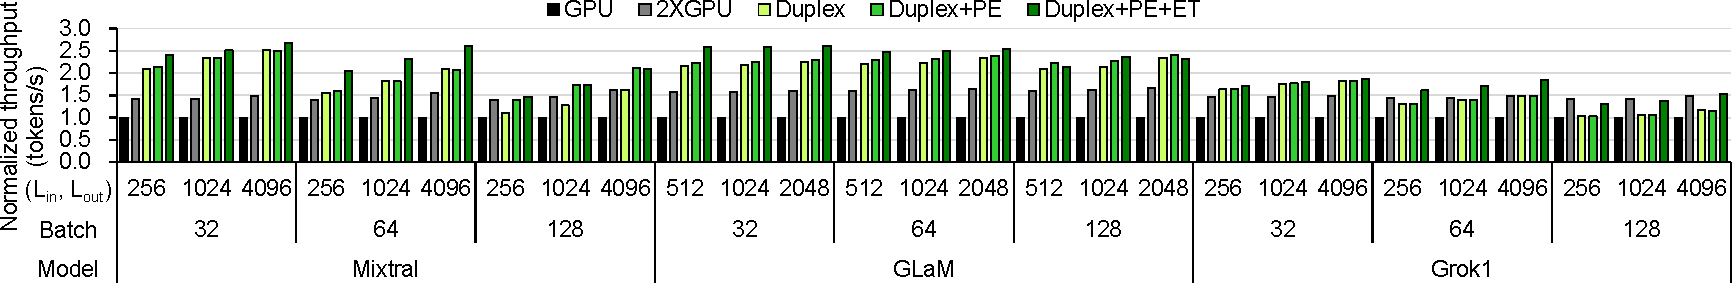
\includegraphics[width=1.0\textwidth]{figures/throughput_graph_cam_ready.pdf}
    \vspace{-0.15in}
  \caption{
  The normalized throughput of \mixtral, \glam, and \grok for various (\lin, \lout) from (256, 256) to (4096, 4096), and batch sizes (32--128).}
  \label{fig:speedup_graph}
  \vspace{-0.1in}
\end{figure*}



\begin{figure}[!tb]
  \center
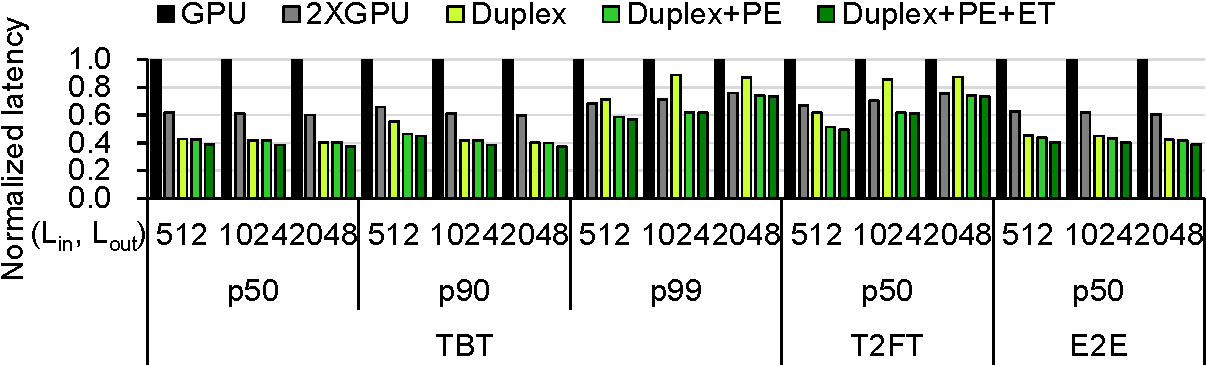
\includegraphics[width=1.0\columnwidth]{figures/eval_latency_bar_cam_ready.pdf}
  \caption{
  The normalized latency (\tbt, \ttft, \ete) of \glam for various (\lin, \lout) from (512, 512) to (2048, 2048) with a batch size of 64.
  }
  \label{fig:eval_latency_bar_graph}
  \vspace{-0.2in}
\end{figure}

To fairly compare the \duplex and GPU, we set the memory capacity of each system to be the same.
With eight or fewer devices, we assume they are interconnected using bidirectional 900GB/s NVLink, similar to an HGX system~\cite{nvidia-hgx}. For configurations with more than eight devices, we assume that each set of eight devices forms a node and that these nodes are interconnected via a system with a 400GB/s Infiniband~\cite{infiniband-whitepaper}.

We developed a cycle-accurate simulator for modeling systems with \duplex and GPUs using Ramulator~\cite{ramulator2-github,cal-2023-ramulator2}.
Our simulator is composed of two main components: a serving scheduler and a cluster.
To support continuous batching, we implemented a serving scheduler that manages ongoing inference requests.
The cluster receives device specifications and system configurations; then, it generates device components.
Based on the model distribution methodology, the simulator distributes model weights across these device components.
The operation of our simulator proceeds as follows:
1) The serving scheduler generates information about the requests being processed at each stage (\eg prefilling or decoding of each request and the current sequence length) and sends them to the cluster.
2) Upon receiving the requests, each device component within the cluster executes the assigned operations and results execution times.
For \lowp, we have modified the Ramulator, specifically the DRAM controllers and internal DRAM behavior models, to enable simultaneous data reading from all banks in the target \bankbundle.
We used the timing parameters of HBM3~\cite{jedec-hbm3} to simulate memory operations in both \duplex and \gpu.
For computing units, the timing data is calculated considering the number and the frequency of the computing units.
The cluster additionally computes the communication time for data movement between devices considering the latency and bandwidth of the HGX system~\cite{nvidia-hgx}, and based on the execution times received from the device components, calculates the final execution times.


We used \mixtral~\cite{arxiv-2024-mixtral}, \glam~\cite{icml-2022-GLaM}, \grok~\cite{grok1}, \opt~\cite{arxiv-2022-opt}, and \llama~\cite{2024-llama3} LLMs for evaluation. 
Mixtral and Grok1 have a structure with all MoE decoder blocks, while GLaM alternates decoder and MoE decoder blocks.
In the MoE layer, Mixtral and Grok1 select two out of eight experts, and GLaM selects two out of 64 experts per token.
To evaluate the performance of \duplex in conventional LLMs without MoE, we also used \opt and \llama.
\mixtral, \grok, and \llama uses GQA, and \glam and \opt uses MHA.
We used FP16~\cite{openai-fp16 ,arxiv-2022-opt} for weight precision.
Considering the number of model parameters, we configured the default number of nodes and the number of devices within each node as follows; \mixtral, \opt, \llama: one node with four devices, \glam: one node with eight devices, \grok: two nodes, each with eight devices.
Unless specified otherwise, we applied the data and job distribution method described in Section~\ref{sec:motivaiton}. 
For \doublegpu, we first increased the number of devices per node to a maximum of eight and increased the number of nodes.
Details of the model configurations are summarized in Table~\ref{tab:model_configuration}.

We used synthesized datasets to quantify the performance improvements of \duplex. 
We sampled the input and output lengths of each request using Gaussian distributions and represented the average of the input and output lengths for the sampled requests.
For expert selection, we chose the target experts for each token using a uniform distribution~\cite{jmlr-2022-switchtransformer}. 
To evaluate the performance in varying queries per second (QPS) situations, we injected requests into the systems following Poisson distributions~\cite{osdi-2022-orca, isca-2024-splitwise, ics-2024-clay} in the experiments shown in Fig.~\ref{fig:eval_qps}.
Otherwise, we assumed that when the inference of a request is finished, the next request is added to the batch and processed together in the next stage using continuous batching.

To measure area overheads and energy consumption, we synthesized the major components of \duplex devices.
We implemented arithmetic units in Verilog and synthesized them using Synopsys Design Compiler with a 7 nm predictive process design kit~\cite{asap7-2016}.
We set the operational frequency of arithmetic units %(FP16 MACs)
of \highp as 1 GHz and \lowp as 650 MHz considering tCCDS of HBM3, which is 1.5 ns.
We modified FinCACTI~\cite{fincacti-2014} to match the published data of SRAM~\cite{isscc-2017-7nm-sram, whitepaper-2018-irds,vlsit-2018-samsung, isca-2021-tpuv4i, isscc-2018-7nm-sram-euv, iedm-2016-tsmc7nm} and used it to model the energy of SRAM-based buffers.
We referred to~\cite{MICRO-2017-fine-grained-dram} for the activation, read, write, and TSV energy of HBM.
We adjusted the area overhead for processing units and buffers on the DRAM die to 1z-nm DRAM technology~\cite{jssc-2022-hynix-hbm3, jssc-2023-samsung-hbm3}.
We then scaled the area overhead by factoring in that the DRAM process has 10$\times$ larger than the logic process for the same feature size~\cite{hotchips-2019-upmem}.

